\clearpage
\section{Trabalho Desenvolvido}
\label{ch:developed}

Esta seção apresenta o trabalho realizado até o momento que auxilia o desenvolvimento 
deste projeto de pesquisa de doutorado. 

%This section presents the work carried out so far that is assisting the
%development of this doctoral research project. \autoref{sec:module} talks about
%some available software tools for performance evaluation and presents the new
%OpenFlow module for simulations. \autoref{sec:scenario} introduces the proposed
%\ac{SDN}-enabled \ac{LTE} simulation scenario, describing its design targets
%and the network topology. Finally, \autoref{sec:controller} describes the
%enhanced OpenFlow controller for the \ac{SDN}-enabled \ac{LTE} network.
% The work presented here is potential precursor of this doctoral research
% project.


%-----------------------------------------------------------------------------%
%\subsubsection{Comparison between the developed works}
%\label{subsec:applications}
%
%In this part, we provide a feature comparison between various state-of-the-art bitrate
%adaptation schemes in each category from the taxonomy in Figure 3.1. Table 3.1 summarizes
%this comparison for each surveyed paper in terms of the following aspects:

%-----------------------------------------------------------------------------%
\subsubsection{Formulação de Programação Linear Inteira~(ILP)}
\label{subsec:applications}

Nós podemos sobrepor uma rede fog-clod multinível para streaming de video e optimizar adaptativamente sua topologia para minimizar a latência de playback e melhorar o tempo de entrega de um video. A programação com reconhecimento de QoE resolve um programa inteiro linear.

Os vértices representam nós de rede e as arestas são os links de rede podendo ser com ou sem fio. Os links podem ser definidos por conexões físicas ou virtuais
Suponha que que existe $n$ usuários conectados na rede e $m$ servidores de streaming de videos, nós queremos encontrar um emparelhamento apropriado entre eles. Um \textit{matching} entre um usuários e um servidor é mostrado como um par $(i,j)$, e é associado com um benefio $a_{ij}$. O conjunto de usuários e servidores são denotados por $U$ e $V$, respectivamente.

\begin{itemize}
\item $\forall (i,j) \in S$, $i \in U$ e $j \in V$.

\item $\forall i \in U$, exite no maximo um par $(i,j) \in S$.

\item $\forall j \in V$, exite no maximo uma tripla $(i,j) \in S$.
\end{itemize}
 
%Com $V$ sendo o conjunto de todos os vertices, definimos uma atribuição $S$ como um conjunto de triplas $(i,j,k)$, considerando a arquitetura da Figura~[1]:

%\begin{itemize}
%\item $\forall (i,j,k) \in S$, $i \in D$ and $j \in U$ e $k \in V$.
%
%\item $\forall i \in D$, exite no maximo uma tripla $(i,j,k) \in S$.
%
%\item $\forall j \in U$, exite no maximo uma tripla $(i,j,k) \in S$.
%
%\item $\forall k \in V$, exite no maximo uma tripla $(i,j,k) \in S$ $\forall i \in M_{D}(i)$.
%\end{itemize}


A programação com reconhecimento de QoS resolve um programa inteiro linear que busca o valor da variável $x_{i,j} (\in (0, 1))$. $x_{i,j}$ é uma variável binária que assume os seguintes valores,

\vspace{0.5cm}
\begin{equation}\label{total_capacity_loss}
x_{i,j} =
\left\{\begin{matrix}
1, & \text{se um usuário \textit{i} é atribuído a um servidor \textit{j}} & \\ 
0, & \text{Caso contrário} & 
\end{matrix}\right.
\end{equation}
\vspace{0.5cm}

Em uma arquitetura multinível, os streamings de video tem um QoE diferente de acordo com os seus requisitos. Por exemplo, streaming em tempo real, como detecção on-line e streaming armazenado, são sensíveis a atrasos. Portanto, esses streamings devem ser processados o mais próximo possível do usuário final, de preferência em nós localizados no primeiro nível da névoa, enquanto que conteudos de video sob Demanda~(VoD) acenitam um atraso maior. Desta forma, vamos identificar cada stream de video requisitado pelos usuários finais por um identificador, a partir de agora simbolizado por "c".
Um nível de servidores, indicado por $S_{c}$, é um conjunto de nós que atende o QoE necessário para fornecer serviços de um stream de video específico, e nós definimos como um intervalo na forma de $S_{c} \in [a, b)$. onde $a_{c} < b_{c}$ e,

\vspace{0.5cm}
\begin{itemize}

\item  $c \in \{1,...,v\}$

\item  $a_{c} = \{a_{1},a_{2},...,a_{v}\}$

\item  $b_{c} = \{b_{1},b_{2},...,b_{v}\}$

\item  $a_{c},b_{c} \in N_{H}$

\end{itemize}
\vspace{0.5cm}

%Para simplificar esta formulação nós estamos considerando que os segmentos de video é requisitado a apenas um servidor fonte, e utiliza um interval de tempo discreto. Assim, $T = {1, ..., T max }$, onde $T_{max}$ é o tempo maximo que o video levaria para executar no nós mais rapido da fog. $T_{max}$ pode ser calculado como 
%
%\begin{equation}\label{minimize}
%T_{max} = \sum^{m}_{k} min(TI_{k | k \in N_{H}})
%\end{equation}

%Para melhor a latência da reprodução do video, nós devemos  minimizar a latencia de um nó para todas requisiçoes de segmentos do video. 

Para simplificar esta formulação nós estamos considerando que os segmentos de video é requisitado a apenas um servidor fonte, bem como o serviço de video streaming já está em execução em seus respectivos servidores. Colocando as limitações abaixo, An initial approach to the QoS-aware schedule is given by the following optimization problem:

\vspace{0.5cm}

%\begin{equation}\label{minimize}
%\text{minimize} \ \ \
%\sum^{\left | D \right |}_{i=1} 
%\sum_{\{j | (i,j,k) \in A\}}
%\sum_{\{k | (i,j,k) \in A\}}
%\frac{ c_{ijk} }{ m_{i}} \ast x_{ijk}
%\end{equation}

Maximizar

\begin{equation}\label{maximize}
\sum_{i \in U} 
\sum_{j \in S_{c}}
a_{ij} \ast x_{ij}
\end{equation}

Sujeito a

\begin{equation}\label{bound_1}
\sum_{\{j | (i,j,k) \in A\}}
\sum_{\{k | (i,j,k) \in A\}}
x_{ijk} = 1,  \forall i \in D
\end{equation}

\begin{equation}\label{bound_1}
\sum_{\{j | (i,j,k) \in A\}}
\sum_{\{k | (i,j,k) \in A\}}
x_{ijk} \leq 1,  \forall j \in U
\end{equation}

\begin{equation}\label{minimize}
\sum_{i \in U} 
\sum_{j \in S_{c}}
bw_{j} x_{ij}
\leq Bw_{j}
\end{equation}

\begin{equation}\label{minimize}
x_{ij}  \in  \{0, 1\}, \forall i \in U,j \in S_{c}
\end{equation}
\vspace{1.2cm}

Para melhorar o desempenho da rede, nós devemos atribuir todos os usuários aos respectivos streaming de video afim de maximizar o benefio total.
%A função objetivo minimiza o makepan do aplicativo fornecido por um planejamento.
%Para melhorar a latência da reprodução do video, nós devemos  minimizar a latencia de um nó para todas requisiçoes de segmentos do video. 
Logo, a função objetivo busca essa mximização. A primeira restrição requer que cada usuário seja atribuído a exatamente um servidor. A segunda restrição garante que cada usuário seja atribuído a no maximo um servidor. Afirma também que, se o número de usuários são maiores do que o número de lostas de download , alguns dos slots de upload permanecem sem atribuição. A terceira restrição garante que os slots de download em uma similaridade com a classe de download diferem de segmentos de video requisitados.

A restrição (6) evita a atribuição de mais um matching do que a capacidade de banda total disponível para cada servidor.

%-----------------------------------------------------------------------------%
\subsubsection{Formulação de Programação Linear Inteira~(ILP)}
\label{subsec:applications}


Para implementar os servidores DASH e os usuários que permitem o streaming de video adaptativo, modificamos o  Adaptive Multimedia Streaming com a base de código AMuSt~(AMuSt). 
A estrutura do AMuSt fornece um conjunto de aplicativos para produzir e consumir vídeo adaptável, com base no padrão DASH [2]. A funcionalidade DASH é fornecida pela biblioteca libdash [35], uma biblioteca de código aberto que fornece uma interface para o padrão DASH. Atualmente, libdash é o software de referência oficial do padrão DASH.
We consider that the end-users are interested in a video available in three different representations, Q = \{480p, 720p, 1080p\} with bitrates \{1750kbps, 3000kbps, 5800kbps\}, respectively, that are a subset of the ones used by Netflix in the past [11]. Each representation is divided into a set of 50 segments, each of a duration of 2 seconds.


\vspace{0.8cm}
\begin{figure*}[htpb]
	\centering
	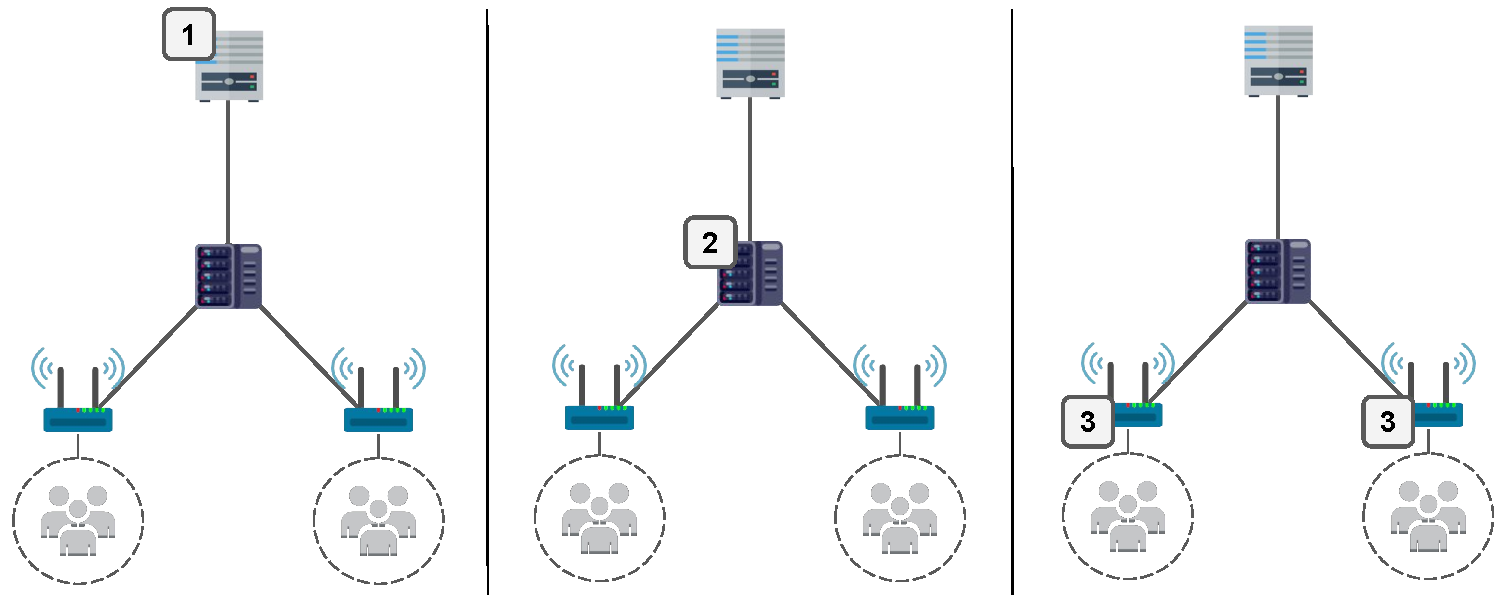
\includegraphics[width=0.75\textwidth]{img/exp-multi-lvl}
% 	\vspace{-1cm}
	\caption{DASH-based Adaptive Multimedia Delivery System for Cloud/Fog Nodes.}
	\label{fig:scenario-arch}
\end{figure*}


Avaliamos o impacto que uma arquitetura multinível de streaming de vídeo adaptativo em uma topologia com tres níveis com um único caminho, apresentada na Fig. 5. Os links possuem comprimento de possui um taxa de dados de 10 MBps e cada AP .


\vspace{0.8cm}
\begin{figure}[htb]
  \centering
    \subfloat[Taxa de bits medio.]
    {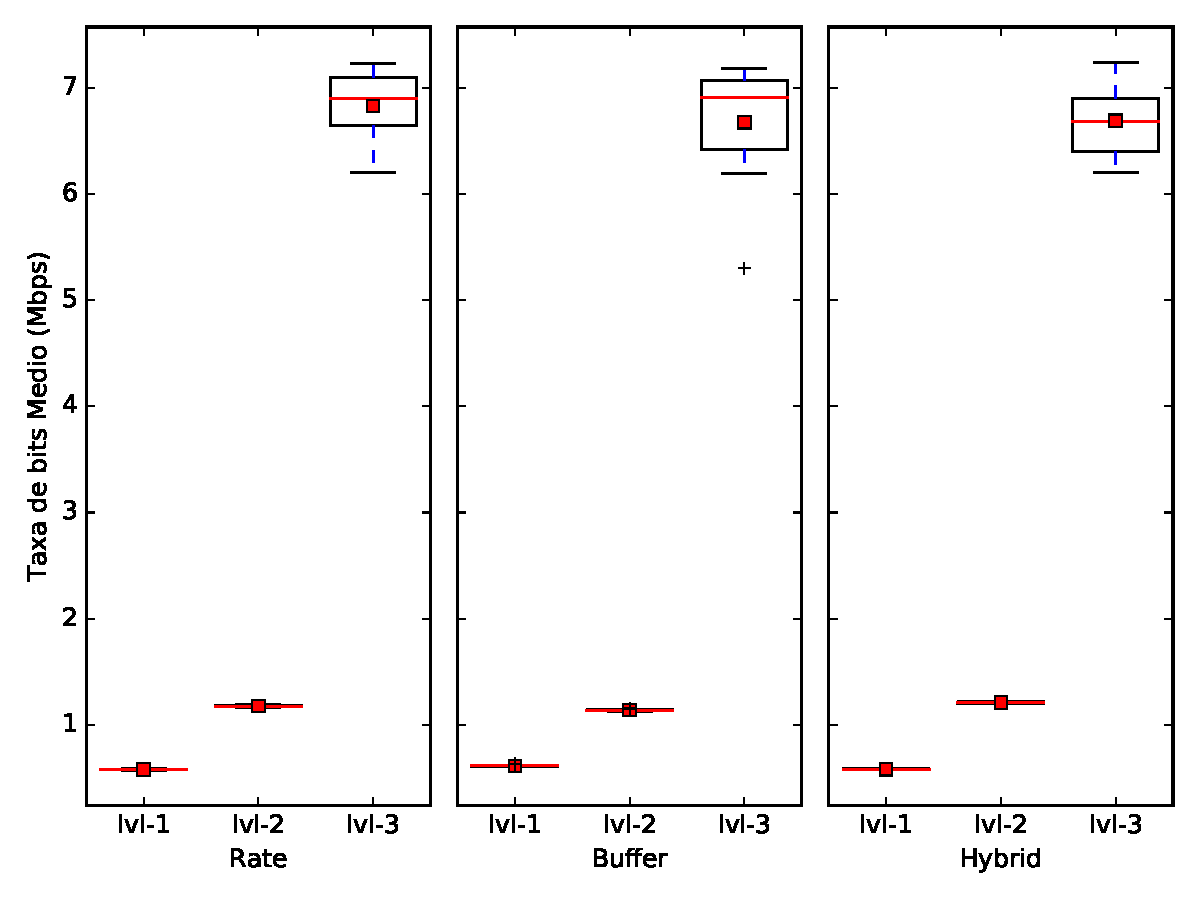
\includegraphics[width=.40\textwidth]{graphs/boxplot-avgBt}
    \label{fig:lte-handover}}
  \hfil \hspace{1cm}
    \subfloat[Tempo total de interrupções.]
    {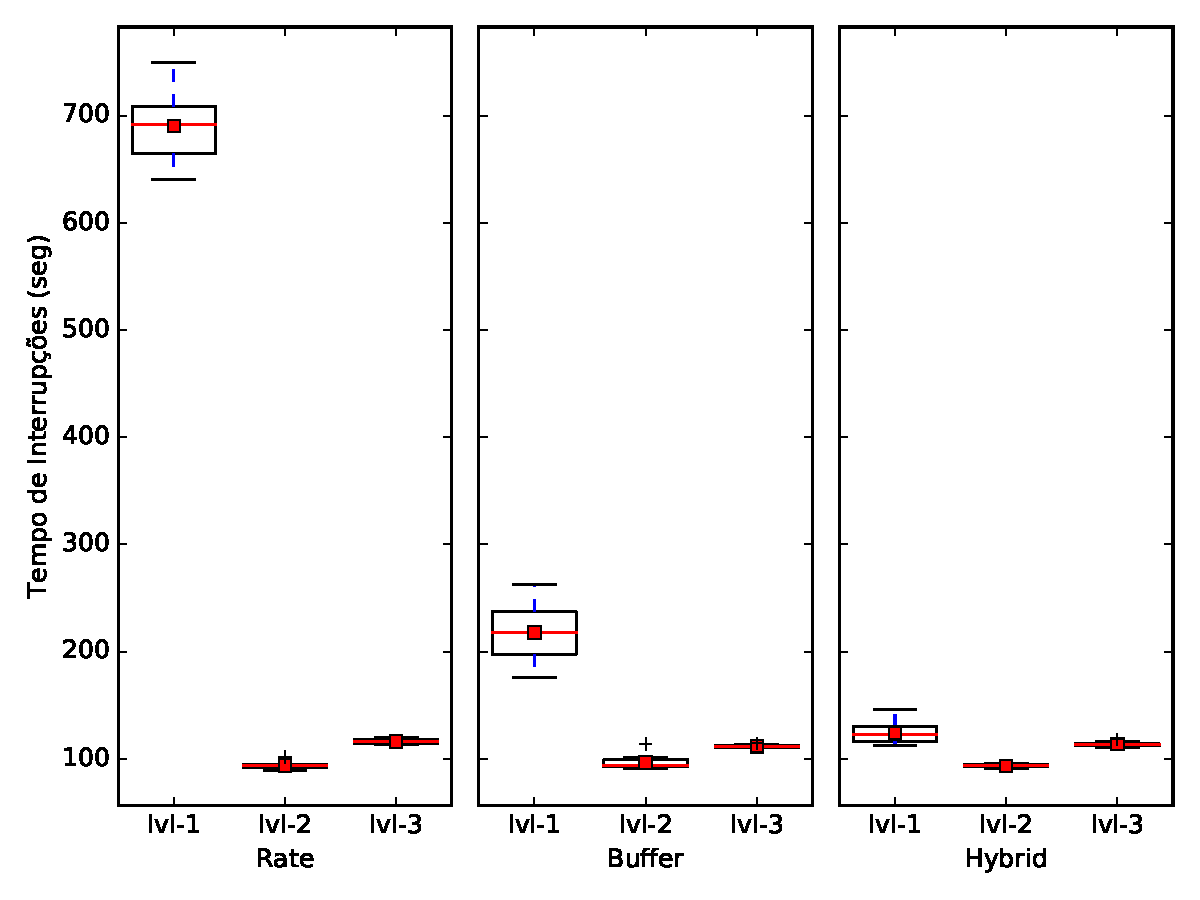
\includegraphics[width=.40\textwidth]{graphs/boxplot-avgStalls}
    \label{fig:dmm-proposal}}
  \caption{Resultados da taxa de bits media e tempo total de interrupções para uma rede com 10 em cada AP.}
  \label{fig:dmm}
\end{figure}

\begin{figure}[htb]
  \centering
    \subfloat[Taxa de bits medio.]
    {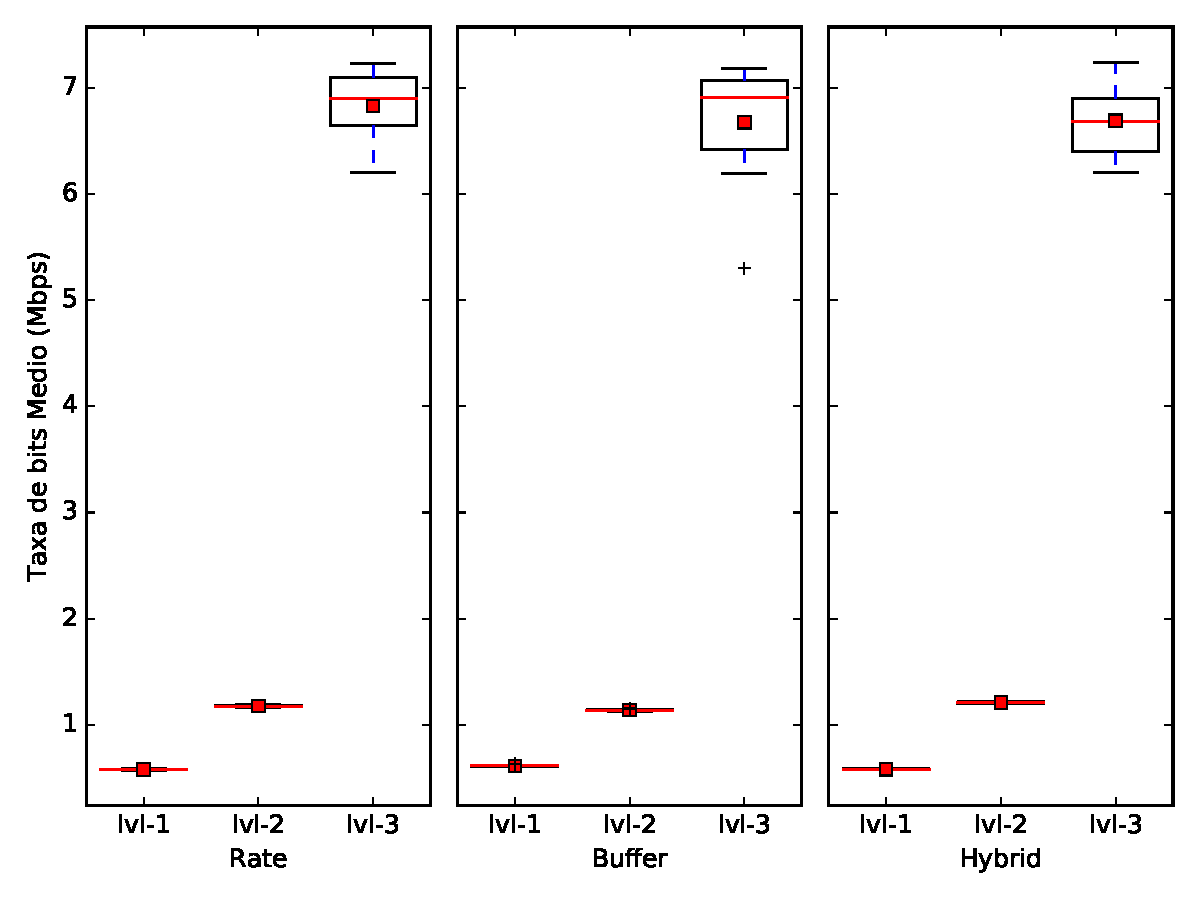
\includegraphics[width=.40\textwidth]{graphs/boxplot-avgBt}
    \label{fig:lte-handover}}
  \hfil \hspace{1cm}
    \subfloat[Tempo total de interrupções.]
    {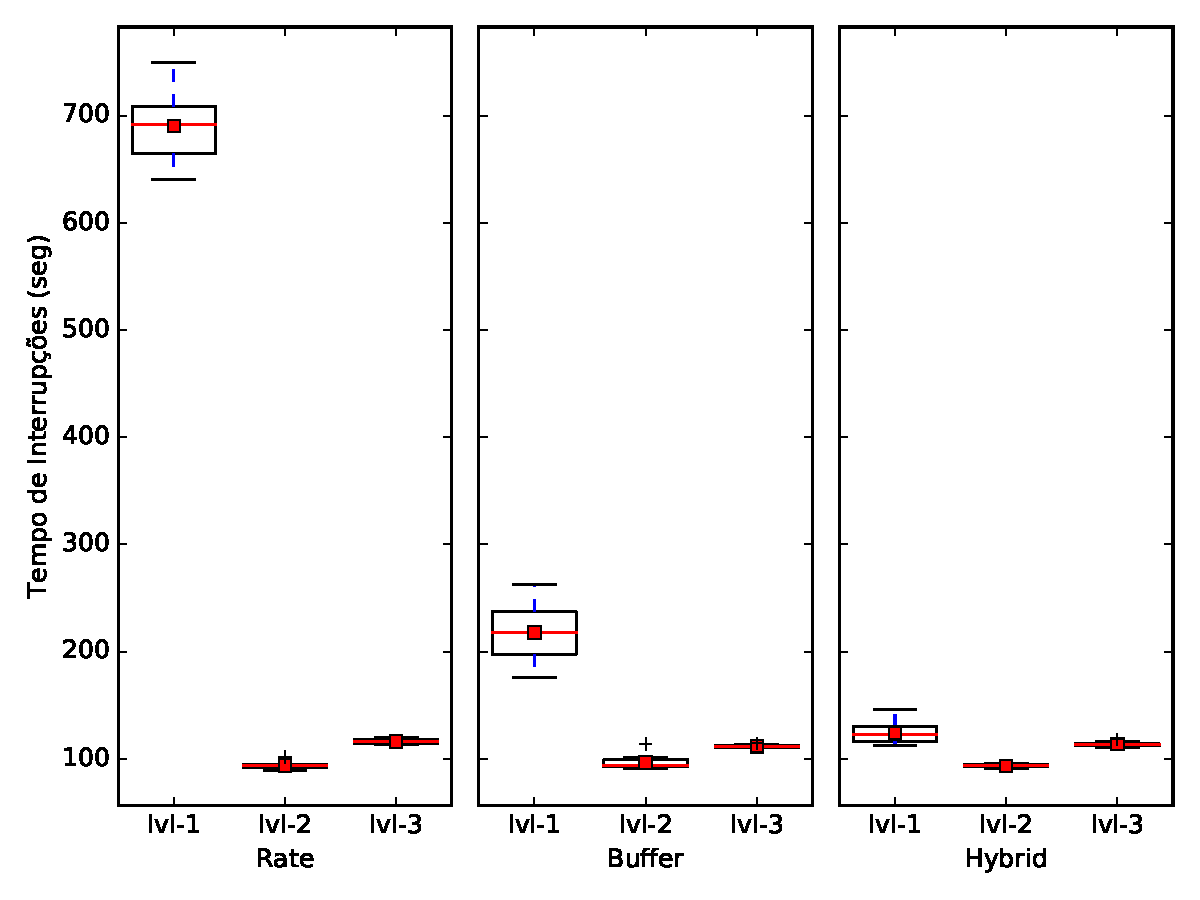
\includegraphics[width=.40\textwidth]{graphs/boxplot-avgStalls}
    \label{fig:dmm-proposal}}
  \caption{Resultados da taxa de bits media e tempo total de interrupções para uma rede com 10 em cada AP.}
  \label{fig:dmm}
\end{figure}